\chapter{Problems with grammars}
\label{chap:problems_with_grammars}

As we could see in previous chapters, it is very easy to write a grammar in a way, that will cause problems once it is imported into MPS.
These problems might occur during creation of any aspect and they are very hard to mitigate.
In this chapter, we will show a few examples of rules, that might cause these problems and try to explain some other effects.
\\

\section{Structural problems}

As a first example, we will describe some problematic structures.
When writing the grammar, it might happen, that we create some patterns, that work just fine with ANTLR parser, but pose problems for the usability of the resulting MPS language.
For example, we might want to use some syntactic sugar such as subrule blocks, which we talked about in section \ref{chap:subrules}.
The problem, that arises here, is similar to the layer problem, we mentioned in section \ref{chap:layer_problem}.
It, however, cannot be resolved automatically.
Let's look at the \parserrule{content} rule of the original XML grammar:

\begin{antlr}
	\parserrule{content} :   \lexerrule{TEXT}? ((\parserrule{element} | \lexerrule{CDATA} | \lexerrule{COMMENT}) \lexerrule{TEXT}?)* ;
\end{antlr}

As we have shown in chapter \ref{chap:whitespaces}, the author of the grammar decided to handle whitespace not by skipping it using ANTLR actions, but rather by wrapping other content with a rule that contains these whitespace characters (the \lexerrule{TEXT} rule).
Then, using the subrule notation, as we can see above, the author made sure, that any content might be eventually wrapped in whitespace or text.
This will enable the parser to handle mixed content (text, comments, tags or CDATA sections) inside an XML tag.
\\

Now let's look, why this poses a problem for us.
In section \ref{chap:subrules}, we have described the way, how we handle subrules.
We unroll them into a set of parser rules and process them in the same way as if they were expanded from the beginning.
The rule above is unrolled to following structure:

\begin{antlr}
	\parserrule{content}          :   \lexerrule{TEXT}? \parserrule{content{\_}block{\_}1{\_}1}* ;
	
	\parserrule{content{\_}block{\_}1{\_}1} :   \parserrule{content{\_}block{\_}1{\_}1} \lexerrule{TEXT}?
	                 ;
	                 
	\parserrule{content{\_}block{\_}1{\_}2} :   \parserrule{element}
	                 |   \lexerrule{CDATA}
	                 |   \lexerrule{COMMENT}
	                 ;		
\end{antlr}

This transformation just translates the shortened subrule notation into a classic parser rule definition, leaving the semantics intact.
\\

When we import this structure inside MPS, the language will not be pleasant to use.
The projectional editor will be full of (most likely) empty \lexerrule{TEXT} placeholders as shown in figure \ref{fig:text_placeholders}.
Sometimes they will contain text, sometimes spaces, but mostly they will distract us and pollute the projectional editor.

\begin{figure}[h]
	\centering
	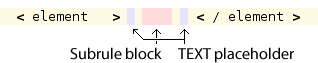
\includegraphics[scale=0.75]{./img/text_placeholders.png}
	\caption{Placeholders in the editor}
	\label{fig:text_placeholders}
\end{figure}

Furthermore, when user wants to insert some content inside an XML tag, he will be forced through two layers and to choose between weird set of some weirdly named block rules, about whose meaning he has no idea.
We can see the process in figure \ref{fig:subrule_problem}.
The auto-completion options represent all end rule alternatives of the artificially created \parserrule{content{\_}block{\_}1{\_}2} subrule.
\\

\begin{figure}[h]
	\centering
	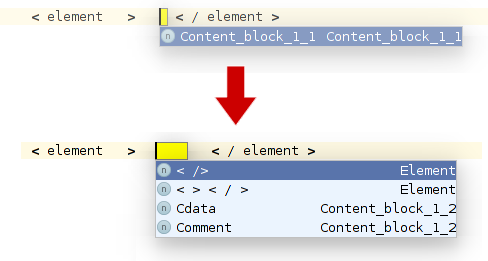
\includegraphics[scale=0.75]{./img/subrule_problem.png}
	\caption{Subrule effect on language usability}
	\label{fig:subrule_problem}
\end{figure}

There is, however, no way, how we could detect or prevent this, when parsing the grammar, since the plugin has no higher understanding of the grammar.
We cannot detect any smart shortcut, like described in section \ref{chap:shortcut_approach}, skipping the first layer of the auto-complete (\parserrule{content{\_}block{\_}1{\_}1}).
The reason is, that the first block rule contains more elements.
Subrules can also be nested inside of each other freely and there can be any setup within multiple levels, additionally with various quantitative operators.
We could of course try to parse the subrule block differently somehow, but for each possible solution, we can always find a very simple case, that will break it.
\\

The easiest solution to this problem is to alter the grammar directly and unroll it manually.
We have done something like that with our SimpleXML language.
We have restructured the content rule into a more simple version:

\begin{antlr}
	\parserrule{content}    :   \lexerrule{TEXT}
	           |   \parserrule{element}
	           |   \parserrule{comment}
	           |   \lexerrule{CDATA}
	           ;
\end{antlr}

It also required us to change the grammar in some other places, but these were just minor changes, mostly concerning cardinality.
It made our MPS language just right, but it also had some bad side effects.
We talk about these side effects further down this chapter in section \ref{chap:problems_with_alteration}.

\section{Other language tweaks}

There are also some cases where we do not have a big structural problem per se, but altering the grammar might yield better MPS language.
We will show one more example where we don't want to improve the structure, but again, the usability of the resulting MPS language.
Let's look at the XML attribute:

\begin{antlr}
	\parserrule{attribute}   :   \lexerrule{Name} \literal{=} \lexerrule{STRING} ;

	\lexerrule{STRING}      :   \literal{"} \regex{~["]*} \literal{"}
	            |   \literal{\textbackslash'} \regex{~[']*} \literal{\textbackslash'}
	            ;
\end{antlr}

The original XML grammar has quotes as a part of the value.
For the resulting MPS language, it would mean that there would be a placeholder for the attribute value, that would expect us to input the leading and trailing quote together with the value too each time.
It would also be marked red unless we enter both quotes inside the value since the regular expression checking for quotes will not match.
The user might be confused by this and won't be able to tell why his string value is incorrect.
\\

In our SimpleXML language, we adjusted the grammar easily in following manner:

\begin{antlr}
	\parserrule{attribute}   :   \lexerrule{Name} \literal{="} \lexerrule{TEXT1} \literal{"}
	            |   \lexerrule{Name} \literal{=\textbackslash'} \lexerrule{TEXT2} \literal{\textbackslash'}
	            ;

	\lexerrule{TEXT1}       :   \regex{~["]*} ;
	\lexerrule{TEXT2}       :   \regex{~[']*} ;
\end{antlr}

We turned quotes into literals and they will only appear in the projectional editor part.
We won't have to write them down each time.
This however has its drawbacks, because user will have to choose, which attribute version he wants to use (single or double quotes?), decreasing the speed with which he could code.
We could also decide to drop one of the two options, but then we will no longer have a full port of the XML language.
Or we could decide to improve the imported language to use one as default and add a special action (for which the intention aspect of the language is used) to switch easily between these two.
It is hard to decide which solution to this problem is the best.
Users might have different intentions, requirements or goals with their MPS language and all approaches lead to some results.

\section{Adjusting grammars}
Above, we concluded, that adjusting the grammar itself might be the only proper solution to some complex situations.
Some of the SimpleXML adjustments, that we put as examples, are simple enough and make the language a lot better.
We also think that the end user of our plugin will be quite educated in this field as they will already be trying to create an MPS language.
It is also expected, that this user will continue on improving the language after the initial import, because the language will just not be as usable without the human touch.
From these reasons, we concluded, that end users of the plugin might also be capable to perform similar grammar adjustments themselves.

\section{Problems with altered grammars [TODO]}
\label{chap:problems_with_alteration}

As stated before, when creating the SimpleXML grammar, we have started off with the original XML grammar\footnote{https://github.com/antlr/grammars-v4/tree/master/xml} and did some adjustments just as described previously.
After that, we ended up with a grammar just good enough for our plugin.
Nonetheless, we noticed that even though the imported language behaves well enough and mimics the XML language quite nicely, the ANTLR parser created from this grammar no longer parses XML successfully.
Some changes we made (e.g. the attribute rule or leaving out parser modes) broke the grammar.
\\

For this, we can blame the ANTLR parser and some dangerous lexer rules.
The greedy way, in which ANTLR matches input on defined tokens and prioritizes their selection, makes some rules (such as \lexerrule{TEXT}) very dangerous, because they swallow a lot more characters than they should.
It is very easy to slip and perform an adjustment that will at first look seem valid inside MPS, but will break the parser.
\\

The reason, why we care about not making the grammar dysfunctional like this, is that if we wanted to proceed with some more complex operations, we would need to automatically generate parsers and use them somehow to parse existing code in that language.
This could be for example utilized within the projectional editor, when detecting layout, or when trying to load existing source code and opening it inside MPS. The user might not even notice that the grammar was damaged or it might have been corrupt from the very beginning. And sometimes we might even wish to break it just for the sake of a better outcome of the import itself (attribute example above). But, advancing further without a valid grammar might make things very complicated.
